\documentclass[11pt]{amsbook}

\usepackage[turkish]{babel}
\usepackage{../Ceyhun}
\usepackage{../amsTurkish}

\begin{document}

\hPage{211}

\begin{figure}[htbp]
\begin{center}
	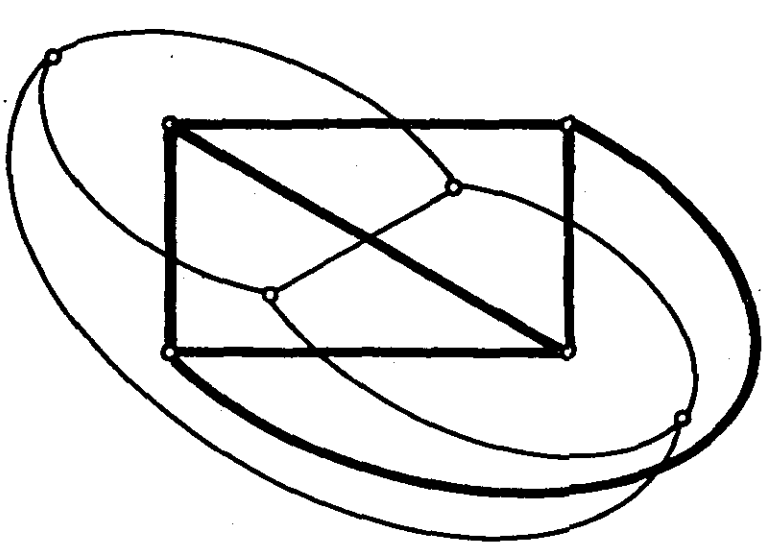
\includegraphics[width = 0.5\columnwidth]{images/ceyhun-211-fig01.png}
	\caption{Özçifteş çizgeye örnek.}
	\label{211-fig01}
\end{center}
\end{figure}

Yukarıda açıkladığımız çizimsel yöntemin gerçekten düzlemsel bir çizgenin çifteşini verdiğinin; $Ç_1$ $Ç_2$ çizgeleri $Ç$ nin iki ayrı çifteşi ise, bu çizgelerin birbirlerine \textit{ikinci düzeyden eşyapılı} olduklarının gösterilmesini okuyucuya bırakıyoruz. Ayrıca $Ç_1$ ve $Ç_2$ çifteş ise, $Ç_1$ in t-kesitleme (t-çevre) matrisi, $Ç_2$ nin t-çevre (t-kesitleme) matrisine özdeştir.

\begin{theorem}
(Whitney) Bir çizgenin çifteşi olabilmesi için gerek ve yeter koşul, çizgenin düzlemsel olmasıdır.
\end{theorem}

\begin{tanit}
\textit{Yeter Koşul:}

Eğer çizge düzlemselse, yukarıda açıkladığımız çizimsel yöntem ile çifteş çizgeyi elde edebiliriz.
\end{tanit}

\end{document}